\documentclass[xcolor=table]{beamer}

\usepackage{arabtex}
\usepackage{utf8}
\usepackage{xcolor}
\usepackage{listings}
\usepackage{todonotes}



\usepackage{tikz}
\usetikzlibrary{shapes.geometric, arrows}
\tikzstyle{process} = [rectangle,rounded corners, minimum width=3cm,text width=10cm, minimum height=1cm, text centered, draw=black, fill=orange!30]
\tikzstyle{arrow} = [thick,->,>=stealth]
\usepackage[sorting=none]{biblatex}
\addbibresource{refs.bib}

\mode<presentation> {
\setcode{utf8}
% The Beamer class comes with a number of default slide themes
% which change the colors and layouts of slides. Below this is a list
% of all the themes, uncomment each in turn to see what they look like.

%\usetheme{default}
%\usetheme{AnnArbor}
%\usetheme{Antibes}
%\usetheme{Bergen}
%\usetheme{Berkeley}
%\usetheme{Berlin}
%\usetheme{Boadilla}
%\usetheme{CambridgeUS}
%\usetheme{Copenhagen}
%\usetheme{Darmstadt}
%\usetheme{Dresden}
%\usetheme{Frankfurt}
%\usetheme{Goettingen}
%\usetheme{Hannover}
%\usetheme{Ilmenau}
%\usetheme{JuanLesPins}
%\usetheme{Luebeck}
\usetheme{Madrid}
%\usetheme{Malmoe}
%\usetheme{Marburg}
%\usetheme{Montpellier}
%\usetheme{PaloAlto}
%\usetheme{Pittsburgh}
%\usetheme{Rochester}
%\usetheme{Singapore}
%\usetheme{Szeged}
%\usetheme{Warsaw}

% As well as themes, the Beamer class has a number of color themes
% for any slide theme. Uncomment each of these in turn to see how it
% changes the colors of your current slide theme.

%\usecolortheme{albatross}
%\usecolortheme{beaver}
%\usecolortheme{beetle}
%\usecolortheme{crane}
%\usecolortheme{dolphin}
%\usecolortheme{dove}
%\usecolortheme{fly}
%\usecolortheme{lily}
%\usecolortheme{orchid}
%\usecolortheme{rose}
%\usecolortheme{seagull}
%\usecolortheme{seahorse}
%\usecolortheme{whale}
%\usecolortheme{wolverine}

%\setbeamertemplate{footline} % To remove the footer line in all slides uncomment this line
%\setbeamertemplate{footline}[page number] % To replace the footer line in all slides with a simple slide count uncomment this line

\setbeamertemplate{navigation symbols}{} % To remove the navigation symbols from the bottom of all slides uncomment this line
}

\usepackage{graphicx} % Allows including images
\usepackage{booktabs} % Allows the use of \toprule, \midrule and \bottomrule in tables

\newcommand{\itodo}[1]{\todo[inline]{#1}} 
\newcommand{\bi}{\begin{itemize}} 
\newcommand{\ei}{\end{itemize}}
\newcommand{\I}{\item} 


%----------------------------------------------------------------------------------------

\title[IE from Ar SMC]{Information Extraction from Arabic Social Media Content } % The short title appears at the bottom of every slide, the full title is only on the title page

\author[R.D.]{Rayan Dankar\\[10mm]
{\small Advisor: Prof. Fadi Zaraket \\
 Committee: Prof. Ali Chehab, Prof. Mohamad Jaber}} % Your name
 
%\institute[AUB] {American University of Beirut}
\institute[AUB]{
\includegraphics[width=2cm]{aubLogo}}
\date{December 17, 2018} 

\begin{document}

\transtrue
\vocalize
%--------------------------------------------------------------
\begin{frame}
\titlepage % Print the title page as the first slide
\end{frame}
%--------------------------------------------------------------
\begin{frame}
\frametitle{Overview} % Table of contents slide, comment this block out to remove it
\tableofcontents 
\end{frame}


%----------------------------------------------------------------------------------------
%	PRESENTATION SLIDES
%----------------------------------------------------------------------------------------

\section {Introduction and background}
\begin{frame}
\frametitle{Introduction \RL{مرحبا}}

%\itodo{one of the top }
%\itodo {official UN languages}

\onslide<2->{
\begin{figure}[!htb]
   \centering
    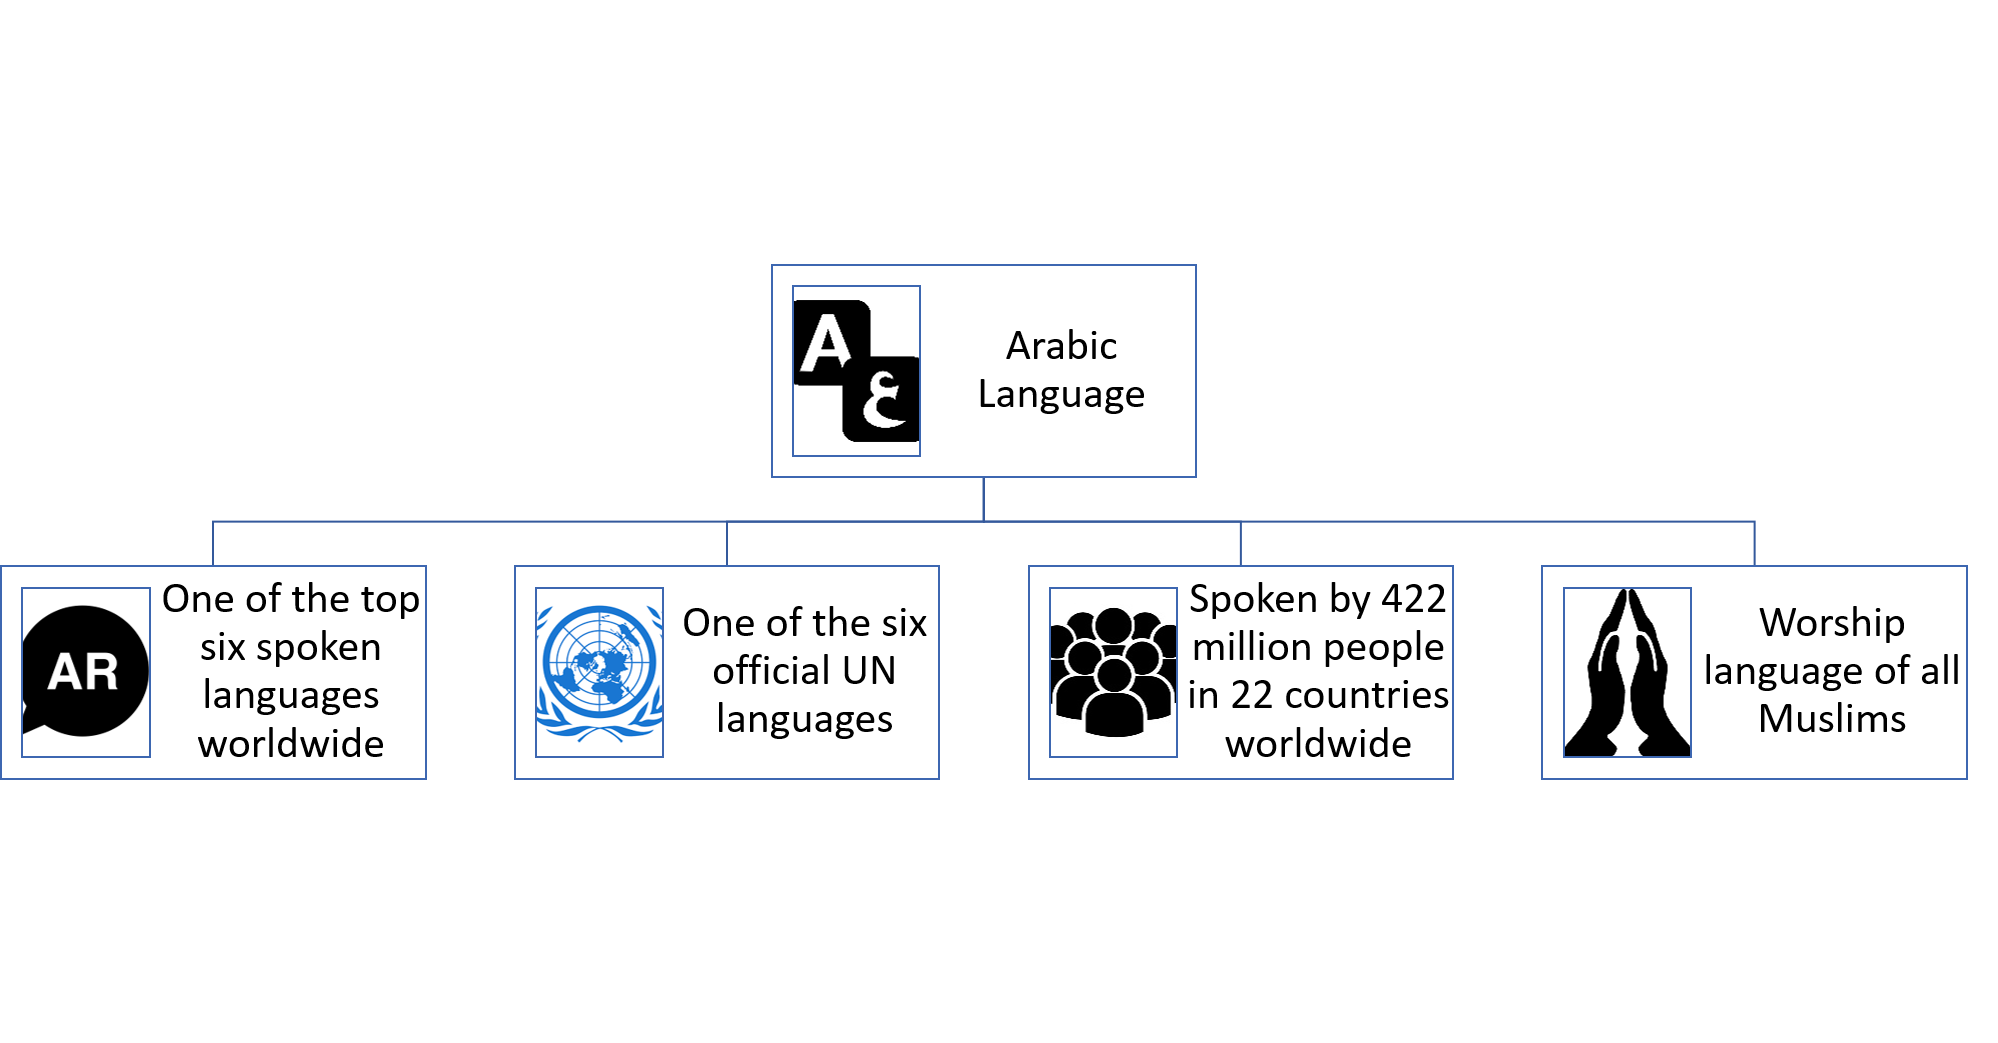
\includegraphics[scale=0.35]{intro.png}
\end{figure}
}
\end{frame}

%------------------------------------------------
\subsection {Modern Standard Arabic (MSA)}
\begin{frame}
\frametitle{Modern Standard Arabic (MSA)}
\begin{itemize}
\item A variant of formal Arabic \RL{فصحى}
\item Common form of Arabic understood by all native speakers
\item Used in formal platforms and events 
%   \bi 
%   \item Such as newscasts, speeches, books and newspapers 
%   \ei 
\end{itemize}
\end{frame}

%------------------------------------------------
\subsection{Arabic Dialects (AD)}
\begin{frame}
\frametitle{Arabic Dialects (AD)}
\begin{itemize}
\item Spoken variations of Arabic 
\begin{itemize}
\item Used in everyday communication and expression
\item Vary across regions
\end{itemize}
\item Examples:
\begin{itemize}
\item Levantine (Lebanon, Syria, Jordan and Palestine), Egyptian
\item Gulf (Kuwait, Bahrain, Qatar, UAE and Oman)
\end{itemize}
\item Differ from {\color{red}MSA} and from {\color{red}each other}
\begin{itemize}
\item along several linguistic features
\end{itemize}
\end{itemize}

\end{frame}

%------------------------------------------------
\subsection*{Linguistic Features of AD}

\begin{frame}
\frametitle{Linguistic Features of Arabic Dialects}

\begin{itemize}[<+->]
\item Alphabet:
    \bi 
    \item \RL{ڤ } represents the phoneme /v/ in loanwords ex: \RL{ڤيينا } Vienna
    \ei 
    \item Phonology: 
    \bi 
       \item \RL{حقوق} (rights) sounds \RL{حوءوء} in Lebanese
    \ei 
    \item Morphology: 
      \bi \I \RL{بديش }, \RL{ما بدي}: negations of \RL{ بدي } (I want)
      \ei 
    \item Orthography
    \bi 
    \I \RL{المجيد}
    \ei
    \item Semantics
    \bi
    \I \RL{ليمون} in Lebanese means oranges and means lemon in Gulf and Egyptian
    \ei
     \item Syntax
\end{itemize}
\end{frame}
%------------------------------------------------
\subsection{Analysis of Social Media Content}

\begin{frame}
\frametitle{Social Media }
\begin{itemize}
\item Widespread use of social media as platforms
\begin{itemize}
\item Socialization: personal events, introductions, reconnecting
\item Communication: user interaction, information exchange
\item Advertisements: engaging customers
\end{itemize}
\item Stakeholders are interested in analysis of content
\end{itemize}

\end{frame}
%------------------------------------------------
\begin{frame}
  \frametitle{ Stakeholders and Possible Questions} 
  
  \bi
  \I Advertisers: how to associate a product with a popular theme
  \I Politicians: what topics interest target demographics
  \I Companies: how to increase brand recognition
  \I Researchers: which posts are useful to extract
  \ei 
\end{frame}


\begin{frame}
  \frametitle{Arabic Social Media Content (SMC)}
\begin{itemize}
\item Arab social media users write multilingual posts
\begin{itemize}
\item MSA 
  \bi  
  \I Often they use Arabic transliterated into Latin (Marhaba) 
  \ei 
\item Arabic Dialects
\item Latin: English, French and others
\end{itemize}
\item Analysis should consider dialects as well
\end{itemize}
%\includegraphics{img0001.png}
\end{frame}
%------------------------------------------------

\begin{frame}
\frametitle{Simple Analysis: Trending Topics}
\begin{columns}
 \column{0.54\linewidth}
           \begin{itemize}
    \item Popular on social media platforms
    \item Receives public interest
    \item Allows the identification of the most important topics
    \end{itemize}
        \column{0.42\linewidth}
        \centering
        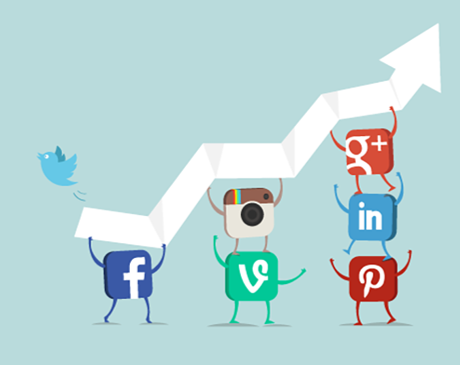
\includegraphics[scale=0.4]{img0003.png}
        
        {\tiny \url{http://expertinreputation.com/wp-content/uploads/2016/07/social-media-trends.jpg}} 
\end{columns}



\end{frame}
%------------------------------------------------


\begin{frame}
\frametitle{Simple Trending Analysis Example }

%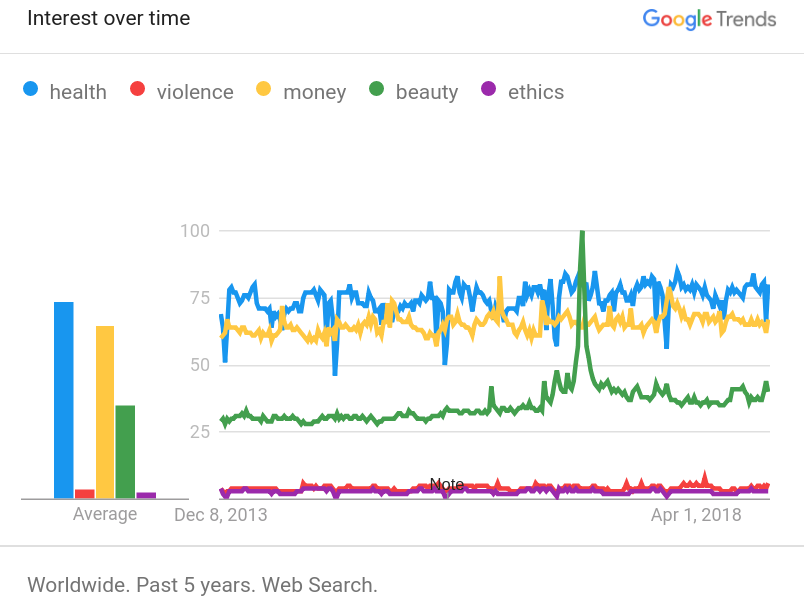
\includegraphics[width=.9\columnwidth]{trends}
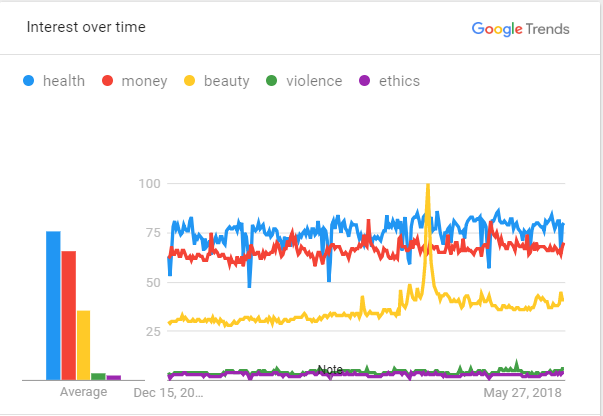
\includegraphics[scale=0.75]{trends2}
\end{frame}
%------------------------------------------------

\begin{frame}
\frametitle{Sophisticated Analysis: Information Extraction}
\begin{itemize}
\item Deeper understanding of social media content
\item Allows network flow analysis
\begin{itemize}
\item Information propagation
\end{itemize}
\item Leverages computational linguistic and graph analysis techniques
\end{itemize}

\end{frame}


%------------------------------------------------

\begin{frame}
\frametitle{Aims of SMC Analysis }

\begin{itemize}
\item Collect data from social media posts
\item Extract entities from posts $V$
\item Extract relation $E \subseteq V \times V$
\item Analyze the extracted graph entities $G=(V,E)$ 
   \bi
   \I In an attempt to answer stakeholder questions
   \ei

\end{itemize}

\end{frame}

%------------------------------------------------
\section{Motivating Example: World Cup Tweet, Missing Journalist}
\begin{frame}
\frametitle{Motivating Example}
\begin{figure}[!htb]
   \centering
    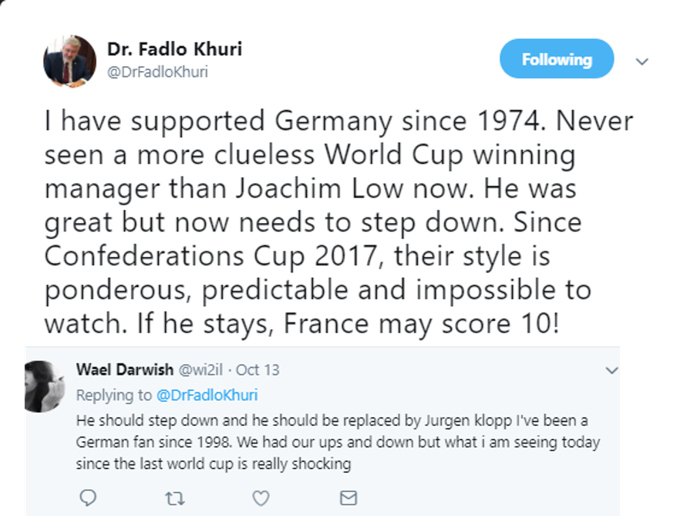
\includegraphics[scale=0.5]{img0004.png}
    
\end{figure}
%\includegraphics{img0005.png}

\end{frame}

%------------------------------------------------

\begin{frame}
\frametitle{Graph Illustration}
\begin{figure}[!htb]
   \centering
    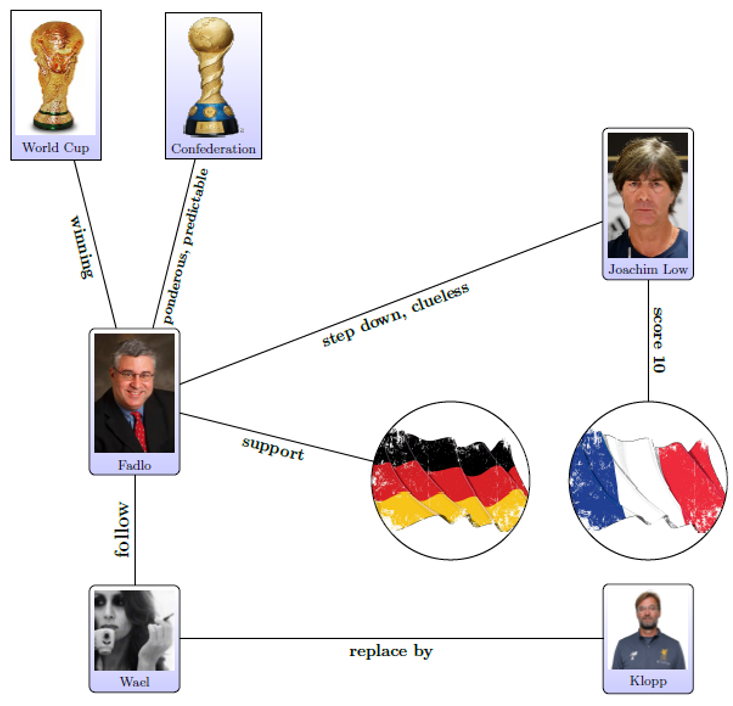
\includegraphics[scale=0.4]{img0008.png}
    
\end{figure}

\end{frame}
%------------------------------------------------
\begin{frame}
\frametitle{Entities and Relational Entities in World Cup Tweet }

  \begin{columns}
    \column{8cm} 
%\begin{table}[]
  \resizebox{.95\columnwidth}{!}{
\begin{tabular}{|l|l|l|}
\hline
\multicolumn{3}{|c|}{\cellcolor[HTML]{C0C0C0}\textbf{Entities}}   \\ \hline
\textbf{person names} & \textbf{country names} & \textbf{objects} \\ \hline
Fadlo Khuri           & Germany                & World Cup        \\ \hline
Wael Darwish          & France                 & Confederation    \\ \hline
Jeurgon Klopp         &                        &                  \\ \hline
Joachim Low           &                        &                  \\ \hline
\end{tabular}
}
%\end{table}
%
%\end{frame}
%------------------------------------------------
%\begin{frame}
%\frametitle{Relational indicators in world cup tweet }
    \column{5cm} 
\onslide<2->{
%\begin{table}[]
\resizebox{.95\columnwidth}{!}{
\begin{tabular}{|l|l|}
\hline
\multicolumn{2}{|c|}{\cellcolor[HTML]{C0C0C0}\textbf{Relations}} \\ \hline
\textbf{verbs}               & \textbf{adjectives}               \\ \hline
follow                       & winning                           \\ \hline
step down                    & ponderous                         \\ \hline
score 10                     & predictable                       \\ \hline
replace by                   & clueless                          \\ \hline
\end{tabular}
%\end{table}
} 
} 
\end{columns}
\end{frame}
%------------------------------------------------

%\begin{frame}
%\frametitle{Motivating Example}
%\begin{itemize}
%\item \textbf{The entities extracted are (nouns: names, objects):} 
%\\ Fadlo, Germany, Wael, Klopp, Joachim Low, World Cup, Confederation, and France.
%
%\item \textbf{The relational entities extracted are (verbs, adjectives and prepositions):}
%\\ follow, support, winning, step down, ponderous, score 10, and replace by
%\end{itemize}
%
%\end{frame}
%------------------------------------------------

\begin{frame}
\frametitle{World Cup Tweet: Entity Annotation }
\begin{figure}[!htb]
   \centering
    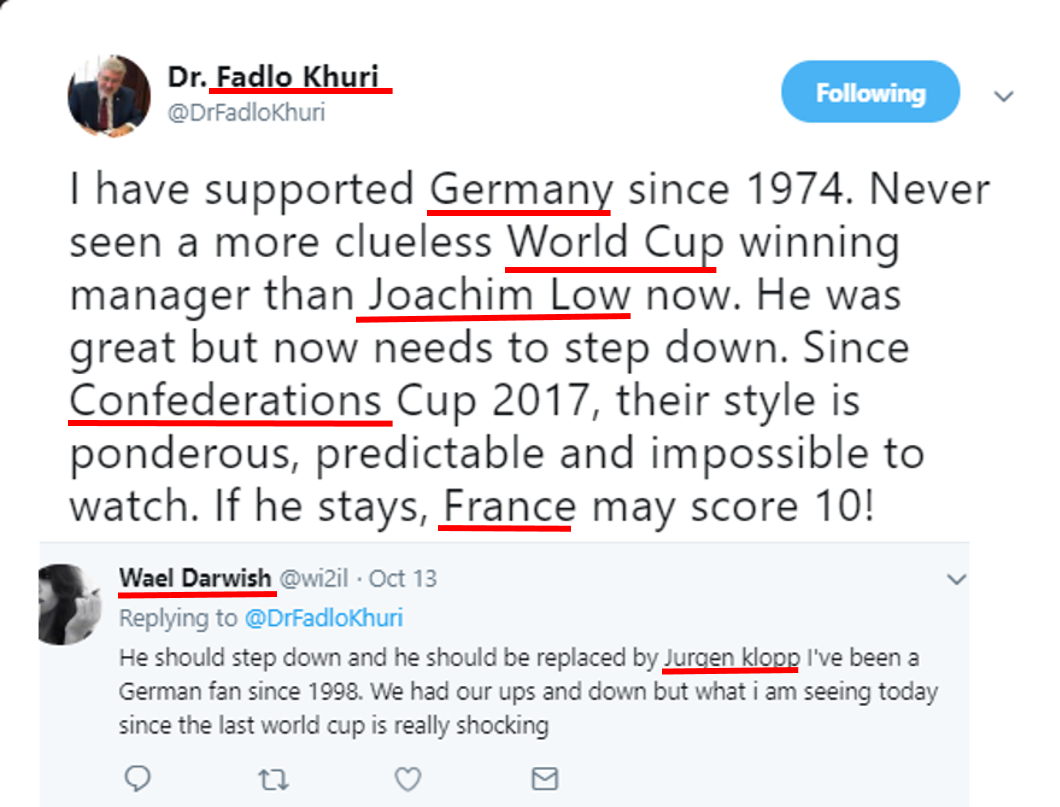
\includegraphics[scale=0.5]{img0004_1.png}
    
\end{figure}
%\includegraphics{img0005.png}

\end{frame}

%------------------------------------------------
\begin{frame}
\frametitle{World Cup Tweet: Relational Entity Annotation }
\begin{figure}[!htb]
   \centering
    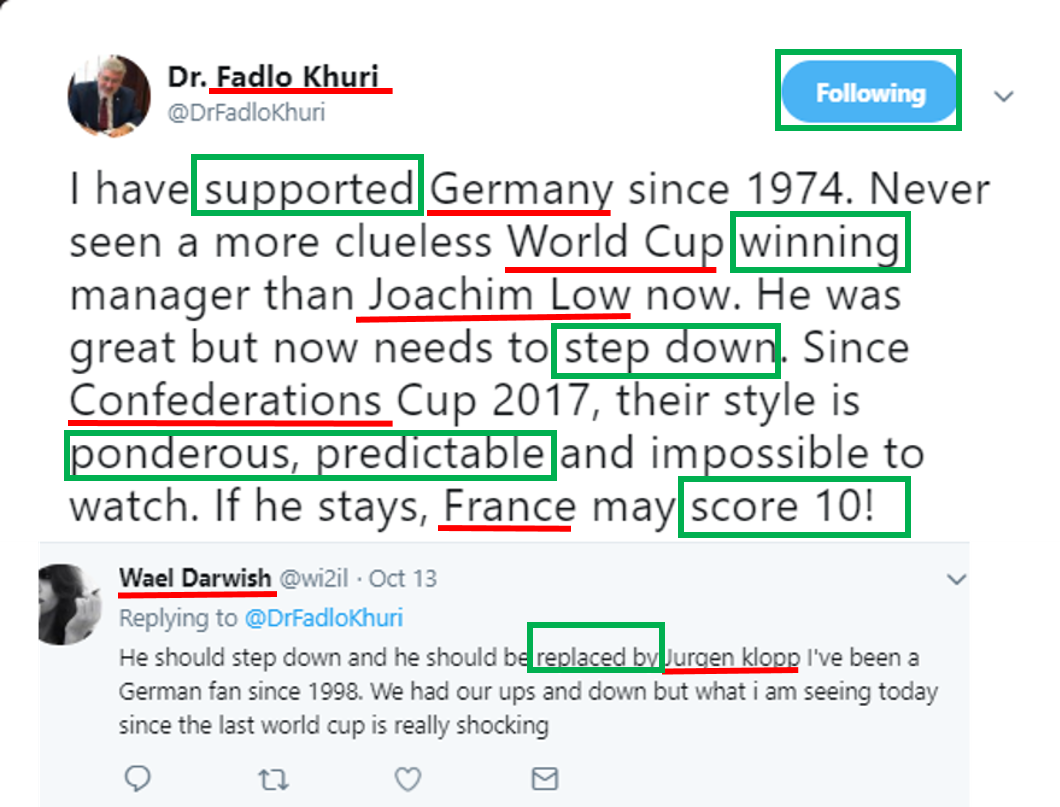
\includegraphics[scale=0.5]{img0004_2.png}
    
\end{figure}
\end{frame}


%------------------------------------------------
%\begin{frame}
%\frametitle{Motivating Example}
% \itodo{Show a table with person names, country names ... they give me entities. Things that give me relations: verbs, ... } 
%  \itodo{Show irsom wa lawin ma3 rayyan.... } 
 % \itodo{Show the graph again. } 
%\end{frame}

%------------------------------------------------
\begin{frame}
\frametitle{World Cup Tweet: Graph Entities }
\begin{figure}[!htb]
   \centering
    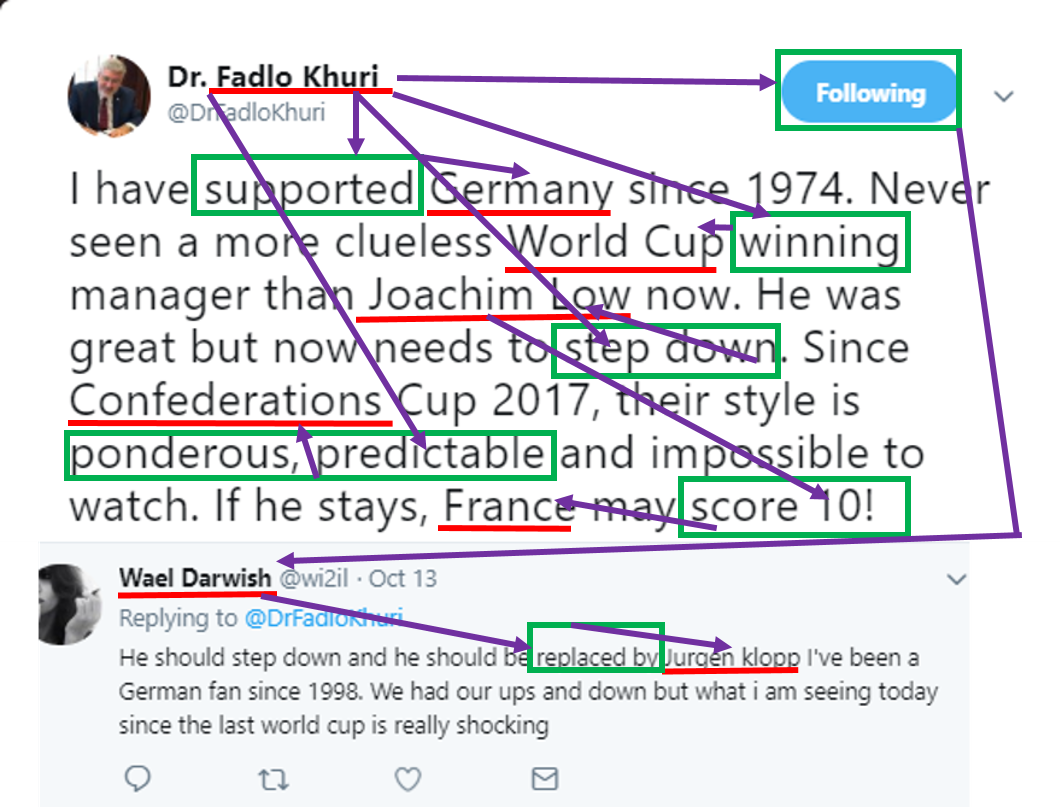
\includegraphics[scale=0.5]{img0004_3.png}
    
\end{figure}
\end{frame}

%------------------------------------------------

\begin{frame}
\frametitle{Knowledge Graph Illustration}
\begin{figure}[!htb]
   \centering
    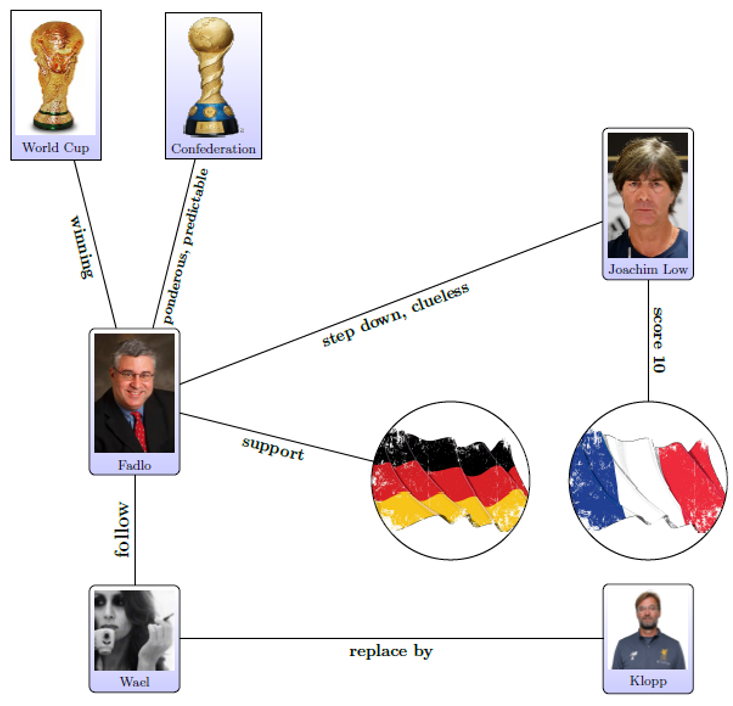
\includegraphics[scale=0.4]{img0008.png}
    
\end{figure}

\end{frame}
%------------------------------------------------

\begin{frame}
\frametitle{Missing Journalist Example }
\begin{figure}[!htb]
   \centering
    
\includegraphics[scale=0.55]{img0009.png}
    
\end{figure}

\end{frame}
%------------------------------------------------
\begin{frame}
\frametitle{Missing Journalist Example: Graph Illustration}
\begin{figure}[!htb]
   \centering
    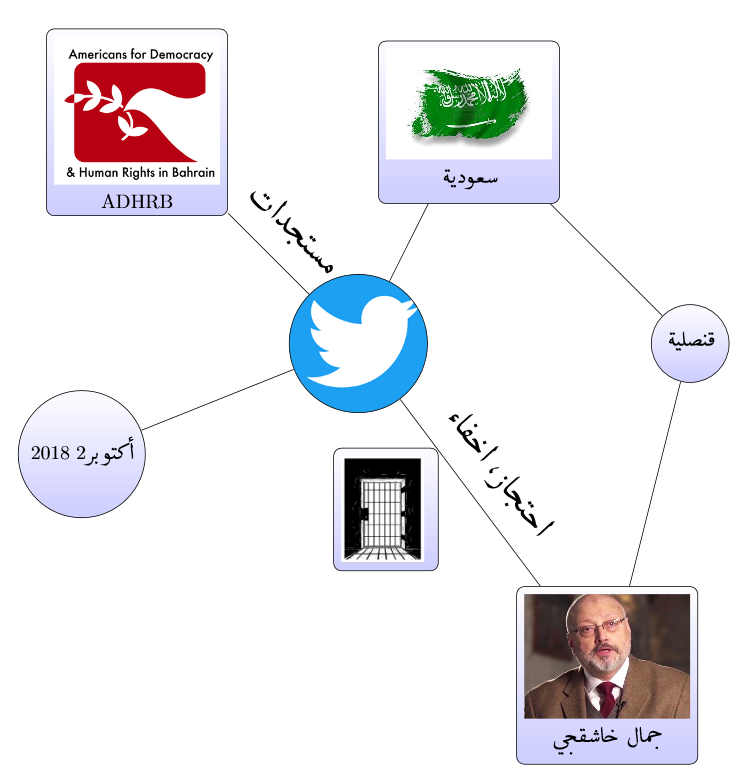
\includegraphics[scale=0.38]{graph2.png}
    
\end{figure}

\end{frame}


%------------------------------------------------
\begin{frame}
\frametitle{Entities and Relational Entities in Missing Journalist Example }

\resizebox{0.99\textwidth}{!}{
\begin{tabular}{|l|l|l|l|}
\hline
\multicolumn{3}{|c|}{\cellcolor[HTML]{C0C0C0}\textbf{Entities}}\\ \hline
\textbf{person names} & \textbf{places} & \textbf{dates}    \\ \hline
\RL{جمال خاشقجي}      & \RL{قنصلية}     & 2018 2\RL{أكتوبر }\\ \hline
ADHRB       & \RL{سعودية}     &                              \\ \hline
\end{tabular}
}
\onslide<2->{
\\[0.4in]
\centering

\begin{tabular}{|c|}
\hline
\rowcolor[HTML]{C0C0C0} 
\textbf{Relational Entities} \\ \hline
\RL{مستجدات}                 \\ \hline
\RL{احتجاز}                  \\ \hline
\RL{إخفاؤه}                  \\ \hline
\RL{تضع}                     \\ \hline
\end{tabular}
}
\end{frame}

%------------------------------------------------
\begin{frame}
\frametitle{Missing Journalist Example: Entities and Relational Entities}

\begin{itemize}
\item \textbf{The entities extracted are:}
\\ ADHRB, \RL{جمال خاشقجي},
\RL{قنصلية},
\RL{سعودية},
2018 2\RL{أكتوبر } 
\\
\item \textbf{The relational entities are:}\\
\RL{مستجدات},
\RL{احتجاز},
\RL{إخفاؤه},
\RL{تضع}
\end{itemize}

\end{frame}

%------------------------------------------------
\begin{frame}
\frametitle{Missing Journalist Example: Entity Annotation}
\begin{figure}[!htb]
   \centering
    
\includegraphics[scale=0.55]{img0009_1.png}
    
\end{figure}

\end{frame}

%------------------------------------------------
\begin{frame}
\frametitle{Missing Journalist Example: Relational Entity Annotation}
\begin{figure}[!htb]
   \centering
    
\includegraphics[scale=0.55]{img0009_2.png}
    
\end{figure}
\end{frame}


%------------------------------------------------
\begin{frame}
\frametitle{Knowledge Graph Illustration}
\begin{figure}[!htb]
   \centering
    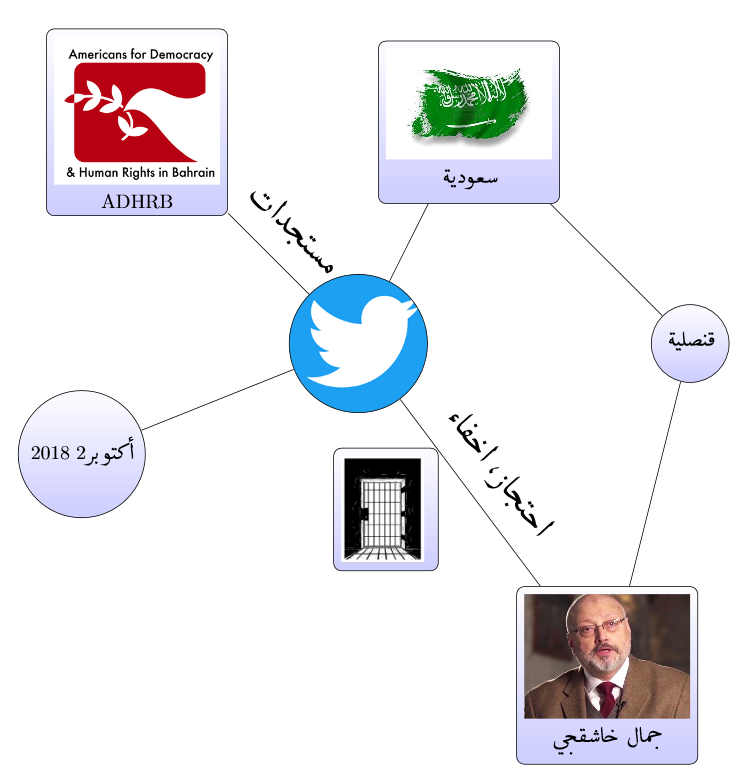
\includegraphics[scale=0.38]{graph2.png}
    
\end{figure}

\end{frame}
%------------------------------------------------
\begin{frame}
\frametitle{Knowledge Graph Aggregation and Cross-referencing} 

\bi
\I Aggregate all unit knowledge graphs into a global knowledge graph
  \bi \I We need cross-referencing for entities and relational entities
  \ei 
\I Information flow analysis across the global knowledge graph
  \bi \I Flow could be across users and their followers or retweeters
      \I Flow could be across topics and sub-topics 
  \ei 
\I Use of rich sub-graphs to dis-ambiguate harder sub-graphs 
  \bi \I Cross-document analysis 
  \ei 
\ei 

\end{frame} 


%------------------------------------------------
\section{Challenges}
\begin{frame}
\frametitle{IE from SMC in Arabic Dialects: Challenges}
\begin{itemize}
\item Lack of resources
\begin{itemize}
\item Corpora
\item Grammars
\item Analysers
\end{itemize}
\item Around {\color{red}5 million} Arabic users on Twitter were recorded by early 2014 \cite{twitter_social}.
\item NLP tools have limited support for MSA and lack support for AD.
\item  Morphological analysers from MSA text exists\cite{Madamira2014, Yamama2016}.
\item Morphological analysers from AD text is still lagging and needs improvement\cite{Madar2018, Guidelines2018, Curras2017}.
\end{itemize}

\end{frame}
%------------------------------------------------
\section{Propose}
\begin{frame}
\frametitle{Propose}
\begin{itemize}
\item A cross-document analysis methodology for Information Extraction including AD content
\item Cross-document NLP studies:
\begin{itemize}
\item coreference of entities in separate documents (relation between two words that have a common referent ex: related by topic).

\item use of the detected cross-references to disambiguate, augment, and integrate the extracted entities and relations.
\end{itemize}
\end{itemize}

\end{frame}

%------------------------------------------------
\begin{frame}
\frametitle{Cross Document Methodology}
\begin{itemize}
\item The methodology requires the construction and the application of the following necessary resources:
\begin{itemize}
    \item Construct computational linguistic models for several dialects 
    \item Extend existing computational linguistic models for existing Arabic dialect models.
\end{itemize}

    \item The computational linguistic models take text as input and return linguistic features such as part of speech, gender, number, voice, stem, and aspect as output.
\end{itemize}
\end{frame}
%\framebreak
%------------------------------------------------
\begin{frame}
\frametitle{Cross Document Methodology}
\begin{itemize}
     \item Develop and use cross-reference metrics to construct relations between the extracted features.
     \item Construct graph theories (entities and relations) and use graph construction techniques to relate the extracted features.
    \item Use graph analysis techniques to analyze the extracted graphs and draw insights from them.
\end{itemize}


\end{frame}
%------------------------------------------------

\section{Background}
\begin{frame}
\frametitle{Background}
\begin{itemize}
\item For this work, our focus is on tweets posted on Twitter.
\item Tweets are messages posted to Twitter platform containing text, images or videos.
\item We aim to:
\begin{itemize}
\item \textbf{collect} tweets from the Twitter platforms
\item extract \textbf{entities} from the tweets
\item extract \textbf{relations} between the extracted entities
\item analyze the entities and the relations using \textbf{graph} construction and analysis techniques 
\item answer questions of interest
\end{itemize}
\end{itemize}

\end{frame}

%------------------------------------------------
\begin{frame}
\frametitle{Background}
\framesubtitle{Twitter API}
\begin{figure}[!htb]
   \centering
    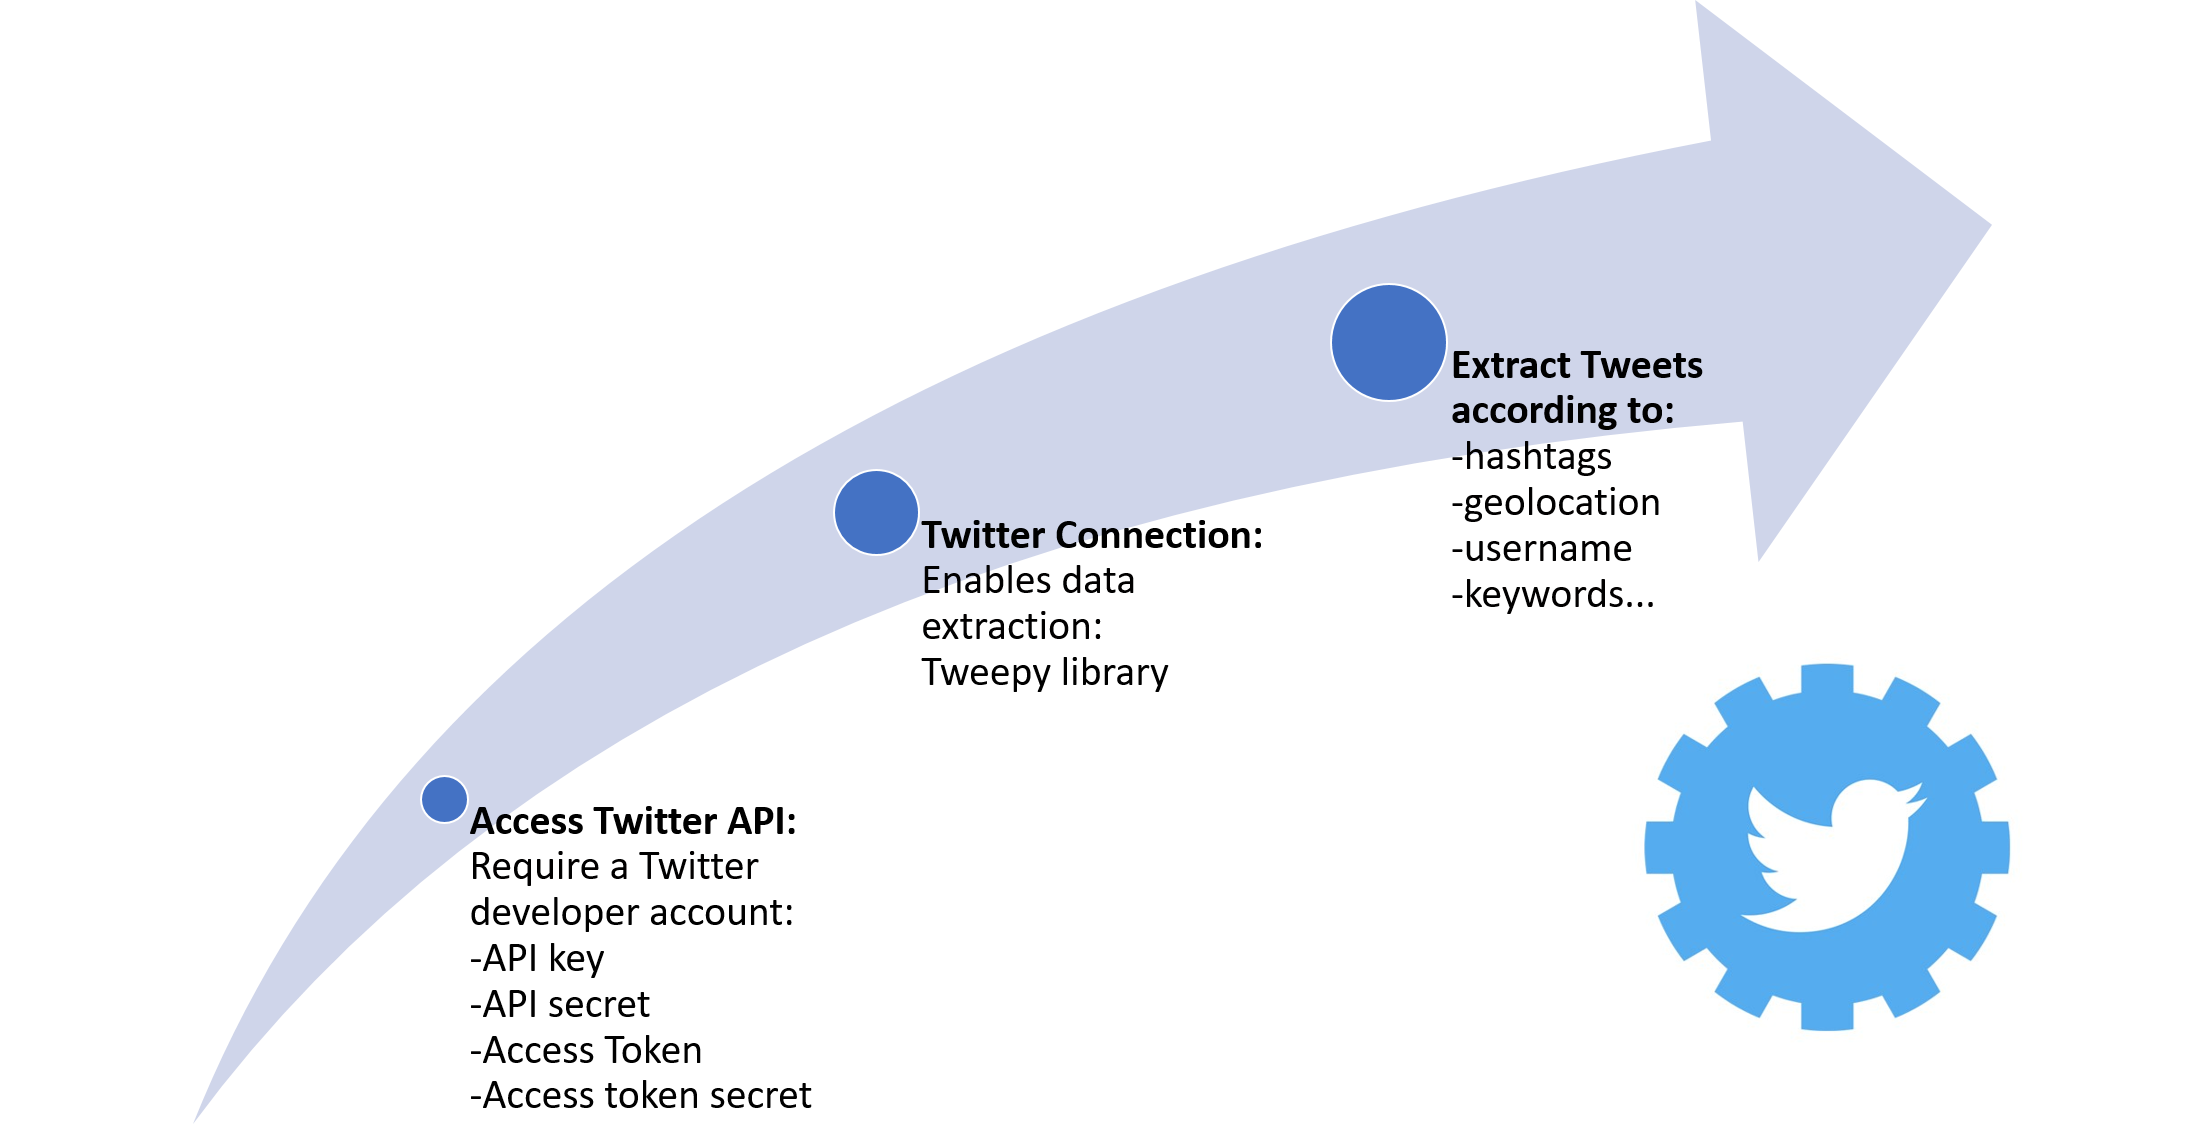
\includegraphics[scale=0.35]{twitter.png}
    
\end{figure}


\end{frame}
%------------------------------------------------

\begin{frame}[fragile]
\frametitle{Background}
\framesubtitle{Twitter API}
\begin{figure}
    \lstset{language=Python}
\lstset{frame=lines}
\lstset{basicstyle=\footnotesize}
\begin{lstlisting}
import tweepy

ckey = 'xxx'
csecret = 'xxx'
atoken = 'xxx'
asecret = 'xxx'

auth = tweepy.OAuthHandler(ckey, csecret)
auth.set_access_token(atoken, asecret)
api = tweepy.API(auth)

maxTweets=100
for tweet in tweepy.Cursor(api.search,q='#peace',
count=100,lang="en",since="2018-10-03").items(maxTweets):
	
	print(tweet.text)
\end{lstlisting}
\caption{python example}
\end{figure}


\end{frame}

%------------------------------------------------
\begin{frame}
\frametitle{Background}
\framesubtitle{Arabic Morphology}
%\includegraphics{img0013.png}
\begin{itemize}
\item Arabic language is morphologically rich and complex.
\item It includes inflectional morphology to express gender, tenses and number.
\item It requires morphological analysis at different levels such as \textbf{tokenization} and \textbf{clitics}.
\end{itemize}

\end{frame}

%------------------------------------------------

\begin{frame}
\frametitle{Background}
\framesubtitle{Tokenization}

\begin{itemize}
\item White space separators between words can be omitted
\bi
\I Due to Arabic letters changing forms according to their position in the word (beginning, middle, end)
\bi
\I Allows the reader to separate words \textbf{visually} rather than relying on the space separation
\ei
\ei



\item \RL{حلواشهية} which means delicious dessert, is a two word fragment: 
\RL{حلوا}
and 
\RL{شهية}
\end{itemize}
\end{frame}
%------------------------------------------------


\begin{frame}
\frametitle{Background}
\framesubtitle{Inflectional Morphology}
\begin{itemize}
\item Expressed in its attachable clitics.
\item \textbf{Several} prefixes and suffixes can attach to the word at the \textbf{same} time.
\item \textbf{\RL{وسيرميها}}
means: and he will throw it, where the attached clitics are:
\item \textbf{\RL{و}}
\item \textbf{\RL{س}}
\item \textbf{\RL{ها}}

\end{itemize}
This inflected word forms a whole sentence on its own.

\end{frame}
%------------------------------------------------

\begin{frame}[<+->]
\frametitle{Background}
\frametitle{Diacritics}
\begin{itemize}
\item Arabic language has optional diacritics
\begin{itemize}
   \item Word \textbf{\RL{عمل}} is an example where adding diacritics changes the tense of the word
\item  \textbf{ \RL{عَمَلٌ} } means the noun work
\item \textbf{\RL{عُمِل}َ} means was done
\item  \textbf{\RL{عَمِل}َ} means worked
\end{itemize}

\item Word\textbf{  \RL{جزر} }is an example where specifying the diacritics changes the whole meaning of the word
\begin{itemize}
    \item \textbf{\RL{جزر} }is interpreted as:
    
    \item \textbf{\RL{جُزُرْ}}
meaning islands or \textbf{\RL{جَزَرْ}} meaning carrots
\end{itemize}
\end{itemize}

\end{frame}
%------------------------------------------------
\section{Entity and Relational Entity Extraction}
\begin{frame}
\frametitle{Entity and Relational Entity Extraction}


In this work computational models will be used to perform entity extraction and relational entity extraction.
\begin{itemize}
\item \textbf{Entity:} term which distinguishes between several items that have similar attributes. Such as: names, locations, and objects.

\item\textbf{Relational Entity:} shows the relation linking between two different entities
\end{itemize}

\end{frame}

%------------------------------------------------

\begin{frame}
\frametitle{Relational Entity Extraction}
\begin{itemize}
\item For the relation entity extraction phase, the analyst sets the expected relations $R=\{r_1,r_2,\ldots,r_{|R|}\}$ 
between the extracted entities.
\item A relation is a tuple $r=\langle e_1,e_2,e_r\rangle$ set by the user where: 
\begin{itemize}
    \item $e_1$ and $e_2\in E $ are entities 
    \item $e_r$ denotes the relation entity label of $r\in R$
\end{itemize}

\end{itemize}
\end{frame}

%------------------------------------------------
\section{Graph Extraction and Analysis}
\begin{frame}
\frametitle{Graph Extraction and Analysis}
A graph $G=(V,E)$ is a graph where:
\begin{itemize}
    \item $V$ represents a set of
vertices
    \item $E$ represents a set of edges
    \item the set of edges are a subset of $V\times V\times L$ where:
    \begin{itemize}
        \item $L$ is the set of labels: $E\subseteq V\times V\times L$
        \item  The entities are represented by $V$ and the relational entities are represented by $E$
    \end{itemize}
    
\end{itemize}  
\end{frame}

%------------------------------------------------

\begin{frame}
\frametitle{Graph Extraction and Analysis}
\framesubtitle{Graph Analytics}
\begin{enumerate}
  \item[1] \textbf{cross-reference:} concerns identifying equivalent graph $G$ elements:
  \begin{itemize}
      \item $v_1 = v_2$ where $v_1$, $v_2 \in V $
      \item $e_1 = e_2$ where $e_1$, $e_2 \in E $
      \item $g_1 \subseteq  G$ and $g_2 \subseteq G$ 
      : $g_1 \equiv  g_2 $
  \end{itemize}
  Equivalence relations between graph elements can be any of the following:
  \begin{itemize}
      \item equal label: =
      \item isomorphism
      \item synonimity
      \item linguistic ontology
  \end{itemize}
  \item[2] \textbf{reachability:} where an entity can reach another entity by a defined relation  %\seti
\end{enumerate}

\end{frame}
%------------------------------------------------

\begin{frame}
\frametitle{Graph Extraction and Analysis}
\framesubtitle{Graph Analytics}
\begin{enumerate}
  
  \item[3] \textbf{important nodes: }where central nodes mean their respective entities are of high degree 
   \item[4] \textbf{hierarchy: }which is displayed by strongly connected components
   \item[5] \textbf{finding network characteristics: }where subnetworks are dense but the whole graph is not
\end{enumerate}

\end{frame}
%------------------------------------------------
\section{Methodology}
\begin{frame}
\frametitle{Proposed Methodology}
\centering

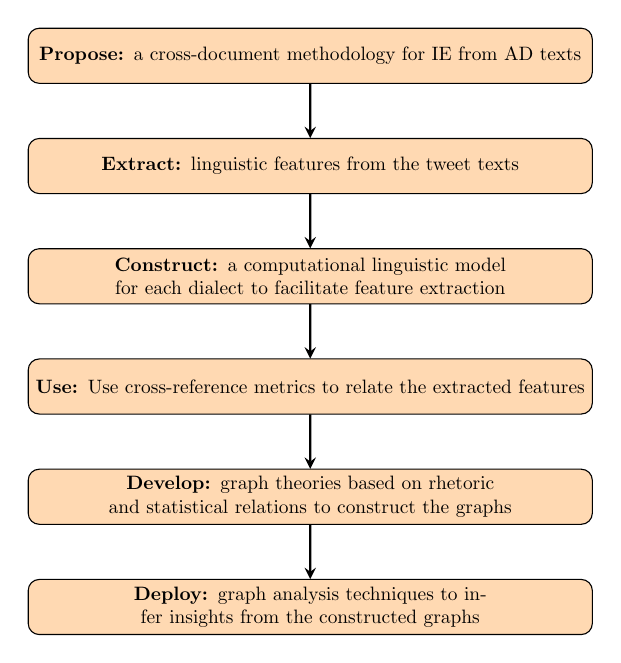
\begin{tikzpicture}[node distance=2cm,scale=0.7,transform shape]
\node (propose) [process] {\textbf{Propose:} a cross-document methodology for IE from AD texts};

\node (extract) [process, below of=propose] {\textbf{Extract:} linguistic features from the tweet texts};

\node (construct) [process, below of=extract] {\textbf{Construct:} a computational linguistic model for each dialect to facilitate feature extraction
};

\node (use) [process, below of=construct] {\textbf{Use:} Use cross-reference metrics to relate the extracted features
};

\node (develop) [process, below of=use] {\textbf{Develop:} graph theories based on rhetoric and statistical relations to construct the graphs
};

\node (deploy) [process, below of=develop] {\textbf{Deploy:} graph analysis techniques to infer insights from the constructed graphs};

\draw [arrow] (propose) -- (extract);
\draw [arrow] (extract) -- (construct);
\draw [arrow] (construct) -- (use);
\draw [arrow] (use) -- (develop);
\draw [arrow] (develop) -- (deploy);

\end{tikzpicture}

\end{frame}
%---------------------------------------------


%------------------------------------------------
\begin{frame}
\frametitle{Proposed Methodology}
\framesubtitle{Construct computational linguistic models for several dialects}
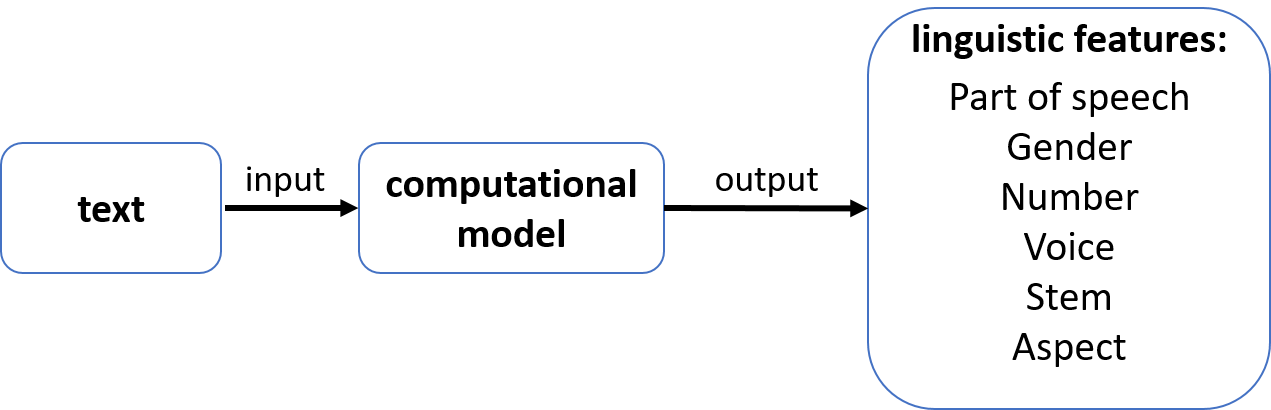
\includegraphics[scale=0.5]{model.png}
\\
\begin{itemize}
\item computational models include phonological, lexical, and morphological features
\item features differ from \textbf{dialect to dialect}
\end{itemize}

\end{frame}
%------------------------------------------------

\begin{frame}
\frametitle{Proposed Methodology}
\framesubtitle{Construct computational linguistic models for several dialects}
%
\includegraphics{img0023.png}
%
\includegraphics{img0024.png}


\textbf{Phonologically:     }
\includegraphics[scale=0.3]{img0022.png}
\begin{itemize}[<+->]
    \item Gulf Arabic pronounces \RL{ق} as /g/~\\ e.g. \RL{قرب} (approach, pronounced as 'garib' in Gulf)
    \item Levantine pronounces it as the glottal stop ('arib)
    \item Gulf Arabic merges \RL{ض} into \RL{ظ}
    \item In Gulf Arabic, \RL{ج} is pronounced as \RL{ي} in many words \\e.g. \RL{دجاج} (chicken) is pronounced as \RL{دياي}
\end{itemize}

\end{frame}
%------------------------------------------------

\begin{frame}[<+->]
\frametitle{Proposed Methodology}
\framesubtitle{Construct computational linguistic models for several dialects}
\textbf{Lexically:   }
\includegraphics[scale=0.3]{img0023.png}
\begin{itemize}
    \item Each dialect has a set of unique words
\end{itemize}

\textbf{Morphologically:   }
\includegraphics[scale=0.3]{img0024.png}
\begin{itemize}
    \item Gulf dialect mostly uses \RL{ب}
 as a prefix to indicate the future tense
 \item Levantine
 dialects use \RL{ راح} or \RL{ ح}
 \item Gulf dialect uses \RL{قعد} to indicate the progressive tense.
\end{itemize}

\end{frame}

%------------------------------------------------
\begin{frame}
\frametitle{Proposed Methodology}
\framesubtitle{Extend existing computational linguistic models for Arabic dialects}
\begin{itemize}
\item Inspect existing models 
\item Enrich them with additional features such as POS and lemmas 
\item Extend dialect lexicons
\end{itemize}
\begin{figure}[!htb]
   \centering
   \begin{tabular} {l|c|c} \\
 Dialect & MSA & Meaning\\ \hline
 
\RL{زنط}& \RL{خنق} & suffocate\\
\RL{زهب}& \RL{جهز} & prepare \\
\RL{زوليه}& \RL{سجادة} & carpet\\
\RL{زيله} & \RL{سلة المهملات }& garbage bin\\
\RL{عوب} & \RL{عنيد}& stubborn \\
\RL{غرشة}& \RL{علبة}& box\\
\RL{نفنوف}& \RL{الفستان}& dress\\
\end{tabular} 
    \caption{Subset of Gulf dialect words}
\end{figure}

\end{frame}
%------------------------------------------------

\begin{frame}
\frametitle{Proposed Methodology}
\framesubtitle{Cross Reference}
\begin{itemize}
\item Use two metrics for cross-referencing terms with their associated linguistic features.\\
\begin{itemize}
\item Semantic distances based on existing dictionaries and digital ontologies.\\
\item Statistical and information theory-based metrics such as distributional similarity.
\end{itemize}
\end{itemize}

\end{frame}
%------------------------------------------------


\begin{frame}
\frametitle{Proposed Methodology}
\framesubtitle{Graph Illustration}
\begin{itemize}
\item A graph  $G=(V,E)$ 
\begin{itemize}
    \item is a set of labels vertices $V$
    \item related with edges $E\subseteq V\times V\times L$
    \item where $L$ is a set of labels
\end{itemize}

\item Each \textbf{vertex} corresponds to an \textbf{entity} term in one or more tweets. 
\item Each \textbf{label} corresponds to a \textbf{relational entity} term in one or more tweets.
\item We will use rhetoric \textbf{relations} extracted from user questions to relate the terms. 
\item We will also use the \textbf{cross-reference} metrics to establish infer relations between the extracted terms. 
\end{itemize}

\end{frame}
%------------------------------------------------


\begin{frame}
\frametitle{Proposed Methodology}
\framesubtitle{Analysis}
After constructing the graph, we will deploy graph analysis techniques to answer user questions
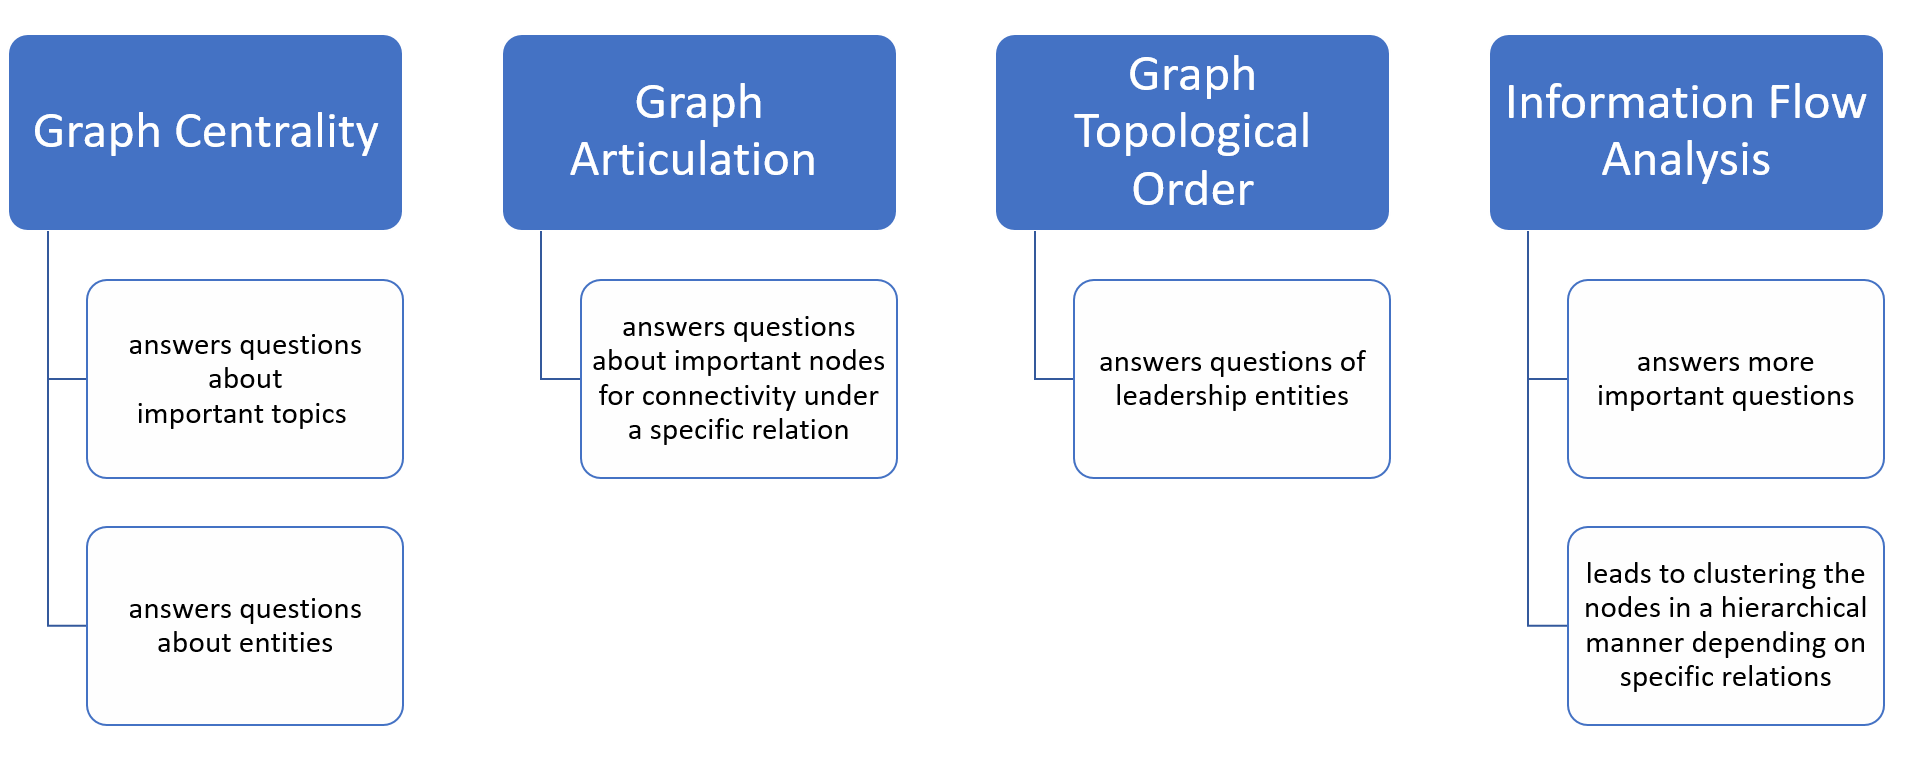
\includegraphics[scale=0.35]{Picture6.png}

\end{frame}
%------------------------------------------------

\begin{frame}
\frametitle{Proposed Methodology}
\framesubtitle{Artificial Intelligence}
Use several artificial intelligence (AI) methods to try and extract the unextracted features.

\begin{itemize}
    \item neural networks (NN)
    \item naive bayesian (NB)
    \item support vector machines (SVMs)
\end{itemize}
\end{frame}

%----------------------------------------------
\section{Plan}
\begin{frame}
\frametitle{Plan}
\resizebox{0.99\textwidth}{!}{
\begin{tabular} {l|ccc|ccc|ccc}

Task & Sep & Oct & Nov & Dec & Jan & Feb & Mar & Apr & May \\ \hline
Related Work & X & X & & & & & \\
Twitter API  & & X & X & & & &  \\
Bahrain Corpus & & X & & & & & & & \\
Relevant Data Collection & & X & X & & & & \\
Relational Entity Extraction & & & & X & X & X &  \\
Graph Construction & & & & X & X & X & \\
Graph Analysis & & & & & & X & X & X \\
Result Combination & & & & & & & X & X & X \\

\end{tabular} 
}
\end{frame}



%----------------------------------------------------------------------------------------

\end{document}